\documentclass[paper=a4, fontsize=8pt]{article}
\usepackage[utf8]{inputenc}
\usepackage[T1]{fontenc}
\usepackage{times}
\usepackage{graphicx}
\usepackage{amsmath,amsfonts,amsthm}
\usepackage{array}
\usepackage{parskip}
\usepackage{fullpage}
\usepackage{enumitem}
\setlist{nolistsep} % for compact lists
\usepackage{hyperref}

%\newlength{\extralength}\setlength{\extralength}{2cm} % if more space is needed
%\addtolength{\textheight}{\extralength}
%\addtolength{\voffset}{-0.5\extralength}

\begin{document}
	\begin{large}\hrule height 1pt
		\begin{tabular}{@{}l@{}} Nerve tracking GUI \\ User manual\end{tabular}\hspace{\stretch{1}}
		\begin{tabular}{@{}r@{}} Version 0.5 \\ April 2020\end{tabular}\hrule	
	\end{large}\par\vspace{\baselineskip}
	
Nerve tracking GUI is used for tracking nerves in volumetric data. The method is the same as used in the paper \emph{Three-dimensional architecture of human diabetic peripheral nerves revealed by X-ray phase contrast holographic nanotomography} by Dahlin \emph{et al.}, Scientific Reports 2020.

Nerve tracking GUI is guided trough keyboard and mouse input. Hints on the basic functionality are written, or appear, above and below the images. The most important functionality is accessed via keyboard inputs in the overview window. This is supplemented by drawing by dragging in the drawing window (see Fig.~\ref{fig:guiscreenshot}). The results are visualized in the 3D visualization window, and can be exported and saved as .obj files (see Fig.~\ref{fig:mousenerves}).

The basic use of the code is: \texttt{nerve\_tracking\_gui(data)}. The format of \texttt{data} and  optional inputs are explained in the help text in the code.

\paragraph{Keyboard input.} Navigation:
\begin{description}
		\item[(Arrow up)] One slice up.
		\item[(Arrow down)] One slice down.
		\item[(Arrow right)] 10 slices up.
		\item[(Arrow left)] 10 slices down.
		\item[(Page up)] 50 slices up.
		\item[(Page down)] 50 slices down.
		\item[(Home)] To the first slice.
		\item[(End)] To the last slice.
\end{description}

\paragraph{Keyboard input.} Functionality:
\begin{description}
		\item[(a)] \underline{A}dd a new nerve by placing a circle. A nerve is added to all slices. The added nerve will become the active nerve.
		\item[(n)] Change the active \underline{n}erve to another already existing nerve. 
		\item[(e)] \underline{E}dit the active nerve in the current slice by dragging the curve.
		\item[(D, d + shift)] \underline{D}elete the active nerve in all slices. Cannot be undone.
		\item[(f)] \underline{F}it the active nerve in the current slice to the image data. This function uses the active setting for edge boundary. %Sometimes good to use multiple times in the same slice.
		\item[(c)] \underline{C}opy the active nerve from the current slice to all subsequent slices. %All subsequent slices will be modified.
		\item[(p)] \underline{P}ropagate the active nerve from the current slice to all subsequent slices. The nerve will be copied and fitted slice-by-slice. The current slice will not be affected. This function uses the active setting for edge boundary. %All subsequent slices will be modified.
		\item[(b)] Change the active setting for a \underline{b}oundary. Toggles between three options: `any', `bright inside', and `dark inside'.
		\item[(s)] \underline{S}ave nerves in a .mat file named NERVES\_XY. Overwrites previously saved nerves.
\end{description}

\paragraph{The suggested workflow.}
Start by getting an overview of the data by navigating through all slices. To add a nerve, navigate to the first slice, then add the curve, fit, and propagate. Navigate through slices to validate the fit. If needed, edit the curve in a slice and propagate. Remember that propagate changes all subsequent slices, so make all edits in order -- starting with the first slice, ending with the last slice. If the fit is not satisfactory in some slice e.g.\ $z$, use copy to duplicate the result from an earlier slice e.g.\ $z-1$. You may or may not edit the curve in slice $z$. Then chose a later slice e.g.\ $z+1$ to initiate propagation. Remember to get back to the first slice in order to add another nerve.    

\vspace{\stretch{1}}\noindent vand at dtu dot dk, 2019, 2020

\newpage
	
	\begin{figure}
		\centering
		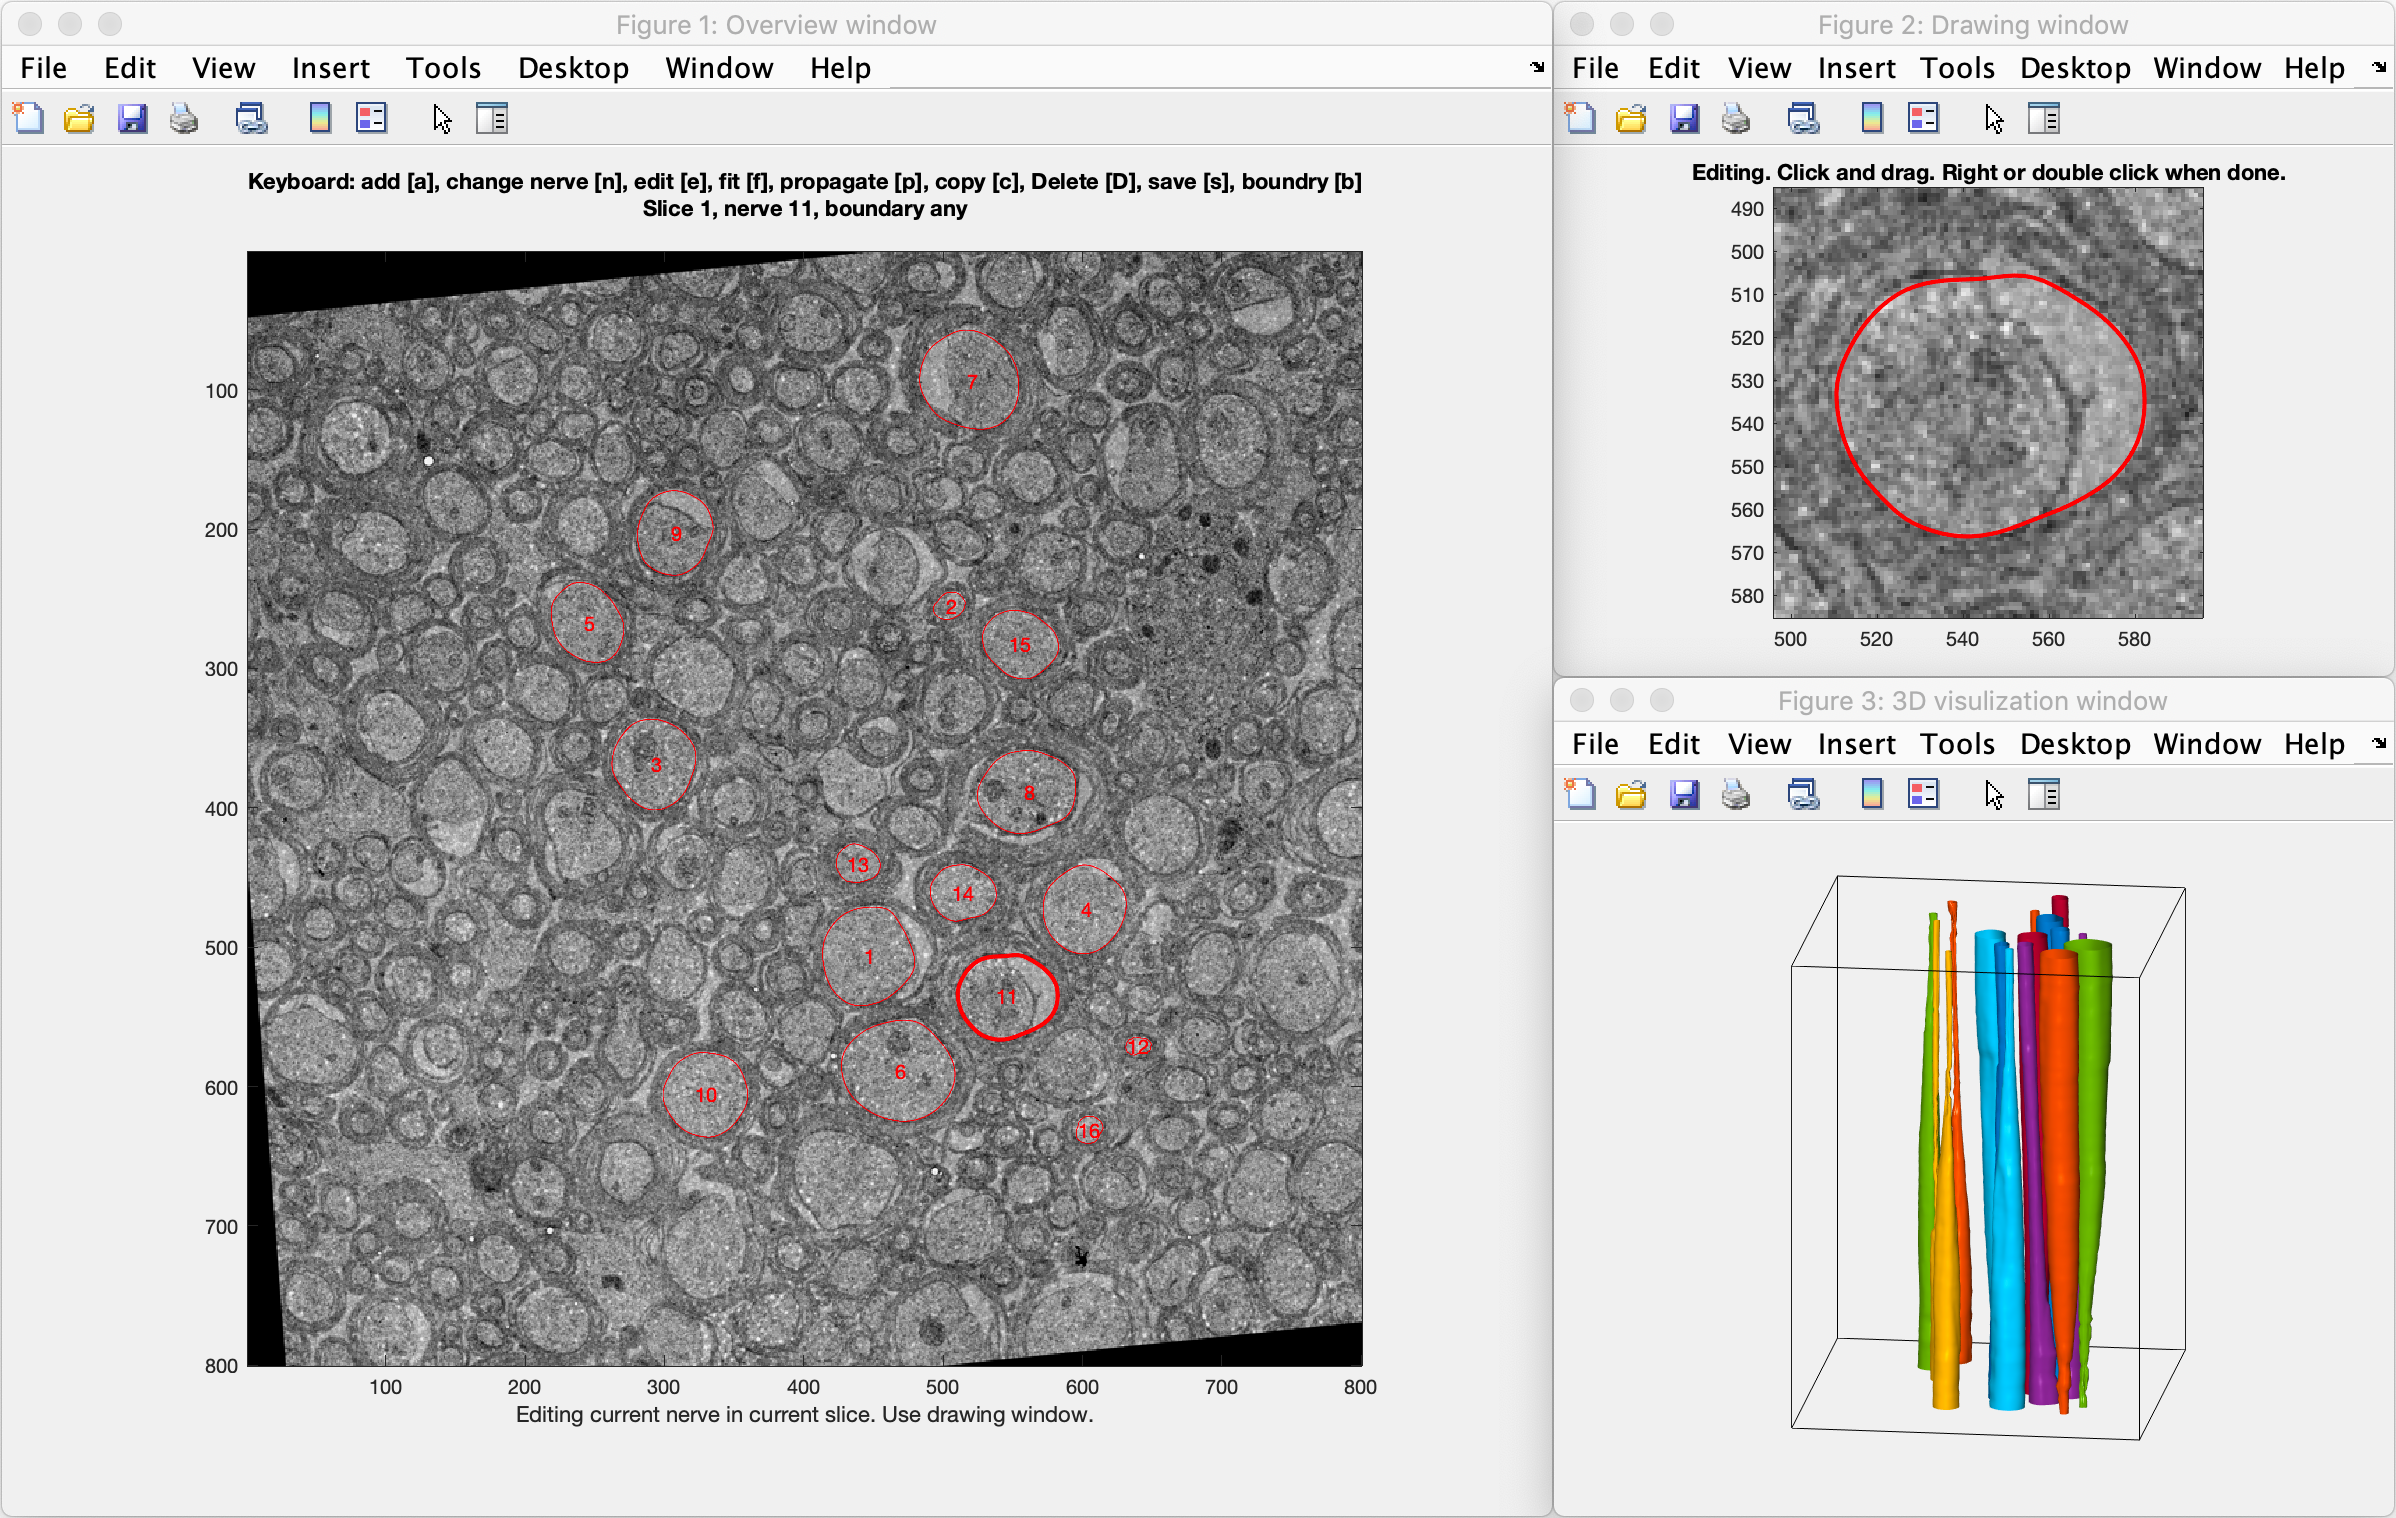
\includegraphics[width=0.9\linewidth]{../images/mouse_nerve_screenshot}
		\caption{A screenshot of the nerve tracking GUI in action. On left the oveview window, on right the drawing window and the 3D visualization window.}
		\label{fig:guiscreenshot}
		\vspace{3\baselineskip}
		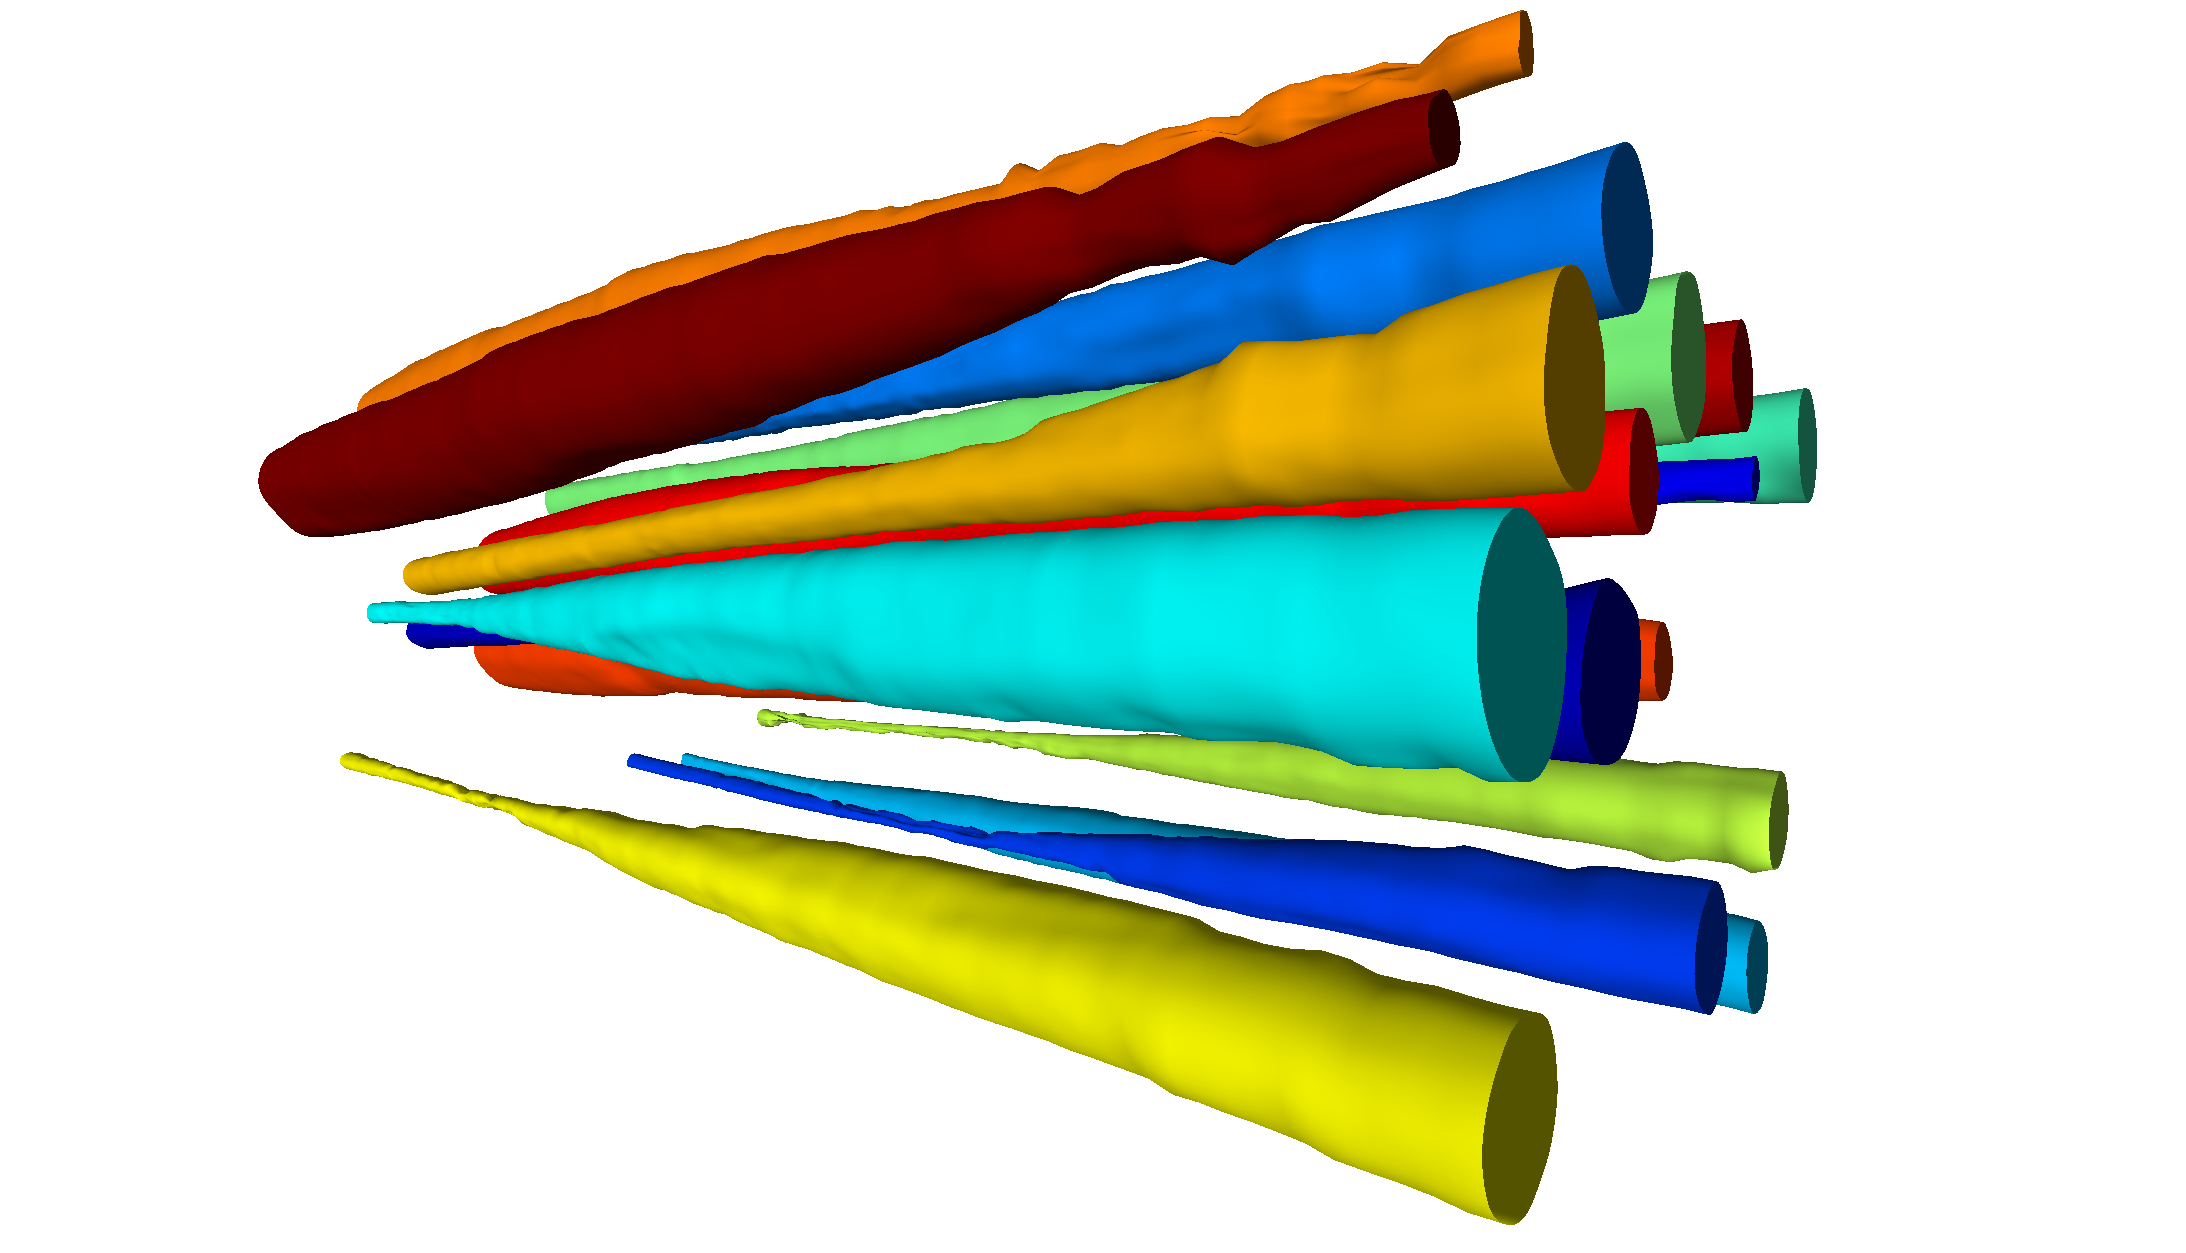
\includegraphics[width=\linewidth]{../images/EM_mouse_meshes_screenshot}
		\caption{An outcome of nerve tracking, in this case saved as .obj file and opened in another program (MeshLab) for the visualization.}
		\label{fig:mousenerves}
	\end{figure}

\end{document}